
\section{Introduction}
In this  Section  i will discuss the  proposed  methodology of this  project this will cover the  following:
\begin{enumerate}
    \item The setup of the raspberry pi
    \item The Data Collection Methods
    \item The Model Development
    \item The Data Analysis Methods
    \item The Ethical Considerations
    \item The validity and reliability 
    \item The Limitations and Delimitation
    \item The timeline
\end{enumerate} 
\section{Setup of raspberry pi}
Firstly once you have  your pi  heres  a  quick  guide to setup the pi are  the following:
\begin{enumerate}
    \item once you unpack the  pi be sure  to  connect keyboard mouse  and hdmi cable
    \item next on a computer you must download the  raspberry pi imager and  selet the  64 bit  recommned os 
    \item once u have os set simpley put the  mircosd card  into  the pi once the  pi is  setup you can make sub dirrys for this project type the  following:
    \begin{verbatim}
        git clone https://github.com/mistaherd/meshnetwork_in_forest.git
    \end{verbatim}
    this  will downlaod the  nessary  eniroment for  setinng up the  pi  intiall this will have to built out  through the  process of  the   project look at the timeline Section
    \item next simply follow the ReadME.md file  to  understand  how  to setup the py
\end{enumerate}



\section{Additional  Research}
In this section will discuss any extra research done on the project.
in this section we will discuss the following:
\begin{enumerate}
    \item ADC
    \item Radio module
    \item Camera
\end{enumerate}
\subsection{ADC}
The MCP3008 was not  available when ordering parts,Another  part for this was choosen which is the  DFR0553 which has the following:
\begin{enumerate}
    \item a supply voltages(VCC) of 3.3 to 5 v
    \item Analog signal  detection 0 to 5v
    \item 4 analog chanel's
    \item resolution of 16 bits
    \item Operating current of 3mA
\end{enumerate}
\subsection{Radio module}
for  this  section we want  to keep  the following in mind :
\begin{enumerate}
    \item We want a module that will send  and  received data
    \item we don't  want  an  expensive solution due  to wanting to  have  multiple nodes
    \item must we pick a standard? 
    \item what module has  an open source project on it 
    \item how do we  set up  a   mesh network with this 
\end{enumerate}
\subsubsection{Do we need a radio standard?}
Lets assume we communicate with two pi via wires  we know that an interference will occur when  we  commutation that is wireless
we can have multiple cases where interference can  occur these are  the following:
\begin{enumerate}
    \item the signal being reflected of objects such as  trees
    \item the signal can reach the  receiver due to an object blocking the antenna
    \item the signal isn't  power to be picked up by the receiver
\end{enumerate}
one essential part of this project is the  ability to have  our nodes have an address to set this up
from a communication preceptive we could develop this when there is open source project that has sorted out the routeing for  you.
only issue with this approach is if there is any issues that come from the open source project we will inheritthene
with this in mind the following standards were found
\begin{enumerate}
    \item LoRa
    \item Zigbee
    \item Sigfox
\end{enumerate}
In \cite{Wu_Liebeherr_2023} lora is used  that will organize sensor
data from all nodes in the spanning tree toward the root(laptop /PC) this can be show by the  following:
\begin{figure}[h!]
    \centering
    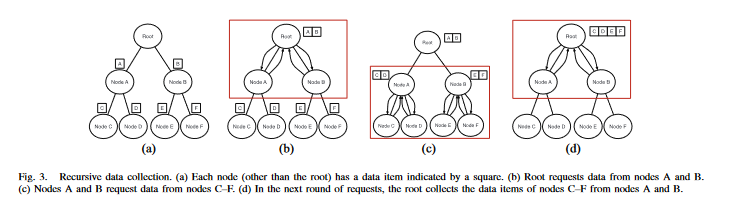
\includegraphics[width=0.5\linewidth]{Images/lora_example_routing_proto.png}
    \caption{protocol Wu used(wu\_lie et.al,2023:16705)}
    \label{protocol Wu used(wu_lie et.al,2023:16705)}
\end{figure}  
this proves it possible  to make a  mesh network useing Lora.
\par 
Lora  
\section{Software Module Development}
this section is here to discuss the method we took  for  developing software  for the  following:
\begin{enumerate}
    \item Sensors 
    \item ADC
    \item Camera
    \item Radio module
    \item Memory management
    \item  TDD
\end{enumerate}
\subsection{Sensors}


\subsubsection{DHT22}

\subsubsection{AS312}


\subsection{ADC}
\subsection{Camera}

\subsection{Memory Mangement}


\subsection{TDD}
Fristly i want to made  some unit tests the aim of this  is the  following:
\begin{itemize}
    \item To make  test  that will be  there for  the  codeing  section of  the  project 
\end{itemize}
this section will discuss the  following for  testing:
\begin{enumerate}
    \item 1 x DHT22
    \item 1 x DFR0026
    \item 1 x AS312
    \item 1 x MM2 Series 900 MHz
    \item 1 x MCP3008
    \item 1 x Raspberry Pi VR 220 Camera
    \item  1 x Li-polymer Battery HAT 
    \item 1 x Turbo 1GB 
\end{enumerate}
\subsubsection{DHT22}
According to the  data sheet \cite{sparkfun} seen as  the data is   8 bits  and  the  range at which this   operates at  -40 to 80$^{o}$c for tempeature
meaning we have  at least  7 bit in the  exponent to  represent  the   measured value.
to represent  the  high  end of this  sensor i used the  following calculation:
$$ 2^6 +2^4 = 80$$ which mean  we have  a 2 bits dedicated to decimal place so the  high temperature to be 80.3$^{o}$c
for the  lowest temp we have 6 bits  to  represent  - 40 due to  2s complement  so lowest  will   be -40.3$^{o}C$
so with that  that  stablish we  must  make a  unit  that will do  the  following:
\begin{enumerate}
    \item Test if the  output is  a float
    \item Test the  high end of  the  temp sensor so it  reads  80.3 as  the highest
    \item Test for the  lowest   temp   around 
\end{enumerate}
be sure to follow  steps  for  folder  setup  follow instructions on page \pageref{folderstructure}.
we get the following sample code:
\begin{lstlisting}[style=mystyle,caption={sample test intial code}]
import unittest
from protest import Read_DHT22
class test_project_code(unittest.TestCase):
    def test_DHT_22_temp_output_type(self):
        self.assertIsInstance(Read_DHT22, float)
    def test_DHT22_temp_range(self):
        self.assertGreaterEqual(Read_DHT22,-30.3)
        self.assertLessEqual(Read_DHT22,80.3)
    
\end{lstlisting} 
This code import unitest . the from protest is  a python files  we can  install  functions from other python files this can be usefull for testing purposes
then we initalized a test class call Unittest.testcase our firstion fucntion of the class  we  check if the number of the output  is a float or not this is  for  testing  tempearture
the next function we test for  is the range i look at the datasheet online   this code is  simpley testing the  limits of the  DHT22
for  humidity  the Datasheet which ranges from 0 to 100 \%
we want to test for the following:
\begin{enumerate}
    \item Test if the  output is  a float
    \item Test if the  output ranges 0 to 100
\end{enumerate}
this lead to the  following code 
\begin{lstlisting}[style=mystyle,caption={sample test for DHT22}]
import unittest
from protest import Read_DHT22
class test_project_code(unittest.TestCase):
    hum,temp=Read_DHT22(2)
    def test_DHT22_output_type(self):
        self.assertIsInstance(Read_DHT22,tuple)
    #....

    def test_DHT22_hum_output_type(self):
        self.assertIsInstance(hum,float)

    def test_DHT22_hum_range(self):
        self.assertGreaterEqual(hum,0.0)
        self.assertLessEqual(hum,100.0)
\end{lstlisting}
seen as we expect our sensor to  print out a humdity and temp values we  set the  output to  a tuple 
to test for this we use isInstacne which will test if its a tuple
next we test for the  limits of the  humidity
\subsubsection{DFR0026 \& MCP3008}
According to the  datasheet \cite{ada} we must keep in mind  that this  componet is  connected to  an ADC 
this  will  give  me  the  following  test conditions:
\begin{enumerate}
    \item Test if  the output is a float

    \item Test  the  range of this  with the  upper limit being 5v 
    \item test the  lover limit being 0 
\end{enumerate}
\begin{lstlisting}[style=mystyle,caption={unit test for  DFR0026 and  MCP3008}]
    import unittest
    from protest import Read_DHT22,Read_MCP3008
    class test_project_code(unittest.TestCase):
    def test_DFR0026_MCP3008_out_type(self):
        self.assertIsInstance(Read_MCP3008,float)
    def test_DFR0026_MCP3008_out_range(self):
        self.assertLessEqual(5.0000000)
        self.assertGreaterEqual(0.0000000)
\end{lstlisting}
this code is in the same in theres of limits
\subsubsection{AS312}
for  this section  we  want our  tests  to  be  the following:
\begin{enumerate}
    \item test for type is boolean 
\end{enumerate}
we can  now add to the snipppet :
\begin{lstlisting}[style=mystyle,caption={unit test for AS312}]
    def test_AS312_out_type(self):
        self.assertIsInstance(Read_AS312,bool)
\end{lstlisting}
\textbf{Note : Don't forget to import read_as12 function from test file}
seen as  thhis is a motion sensor  our ouout will be true or false
\subsubsection{Raspberry Pi VR 220 Camera}
according to the  data sheet \cite{Camera}
we the  resoultion to  it uses is  1080p50 which is 1920x1080p so our  tests will have to  in copoarte  the  followoing:
\begin{enumerate}
    \item Test the  output shape  if open cv is  gonna  be  used 
    \begin{enumerate}
        \item test  the  amout of   elelecelm in the  3 dimesional   array 
    \end{enumerate}
    \item test the  file  type  is png
\end{enumerate}
this would lead me to the following code snippet.
\begin{lstlisting}[style=mystyle,caption={camera unit test}]
    def test_Raspberry_Pi_VR220_out_shape(self):
    self.assertEqual(Read_Raspberry_PiVR220.shape,(1920,1080,3))
\end{lstlisting}
this function check the  pixeal count or resoulkation
\subsubsection{Li-polymer Battery HAT}

\subsubsection{memory moduldes }
in this setion will dicuss the following:
\begin{enumerate}
    \item silicon power 32GB 
    \item Turbo 1GB
\end{enumerate}
for this  i will use  useing  a  bash script(see this on page \pageref{TDD sample bash}) and what we are doing is  testing  the size in a  certain range for the silicon  SD card
\begin{enumerate}
    \item  Turbo 1GB
    as from above we are  import the file at which where our functions live in code frist we import the function
    \begin{lstlisting}[style=mystyle,caption={si powerd SD snippnet }]
        import unittest
        from protest import Read_DHT22,Read_MCP3008,Read_AS312,Read_Raspberry_PiVR220,Read_Memory_module
    
        def Test_memory_module_turbo_1GB_size(self):
            #testing  turbo 1GB
            self.assertLessEqual(Read_Memory_module,1e9)
            self.assertGreaterEqual(Read_Memory_module,0)
    \end{lstlisting}
    then simply we call assert and greater than which sets the bounds of the   modes the 1e9 is a way to put $1 × 10^9$
    whcih output that will between 1GB and  0
    \item silicon power 32GB
\end{enumerate} 
\subsubsection{MM2 Series 900 MHz}

\subsubsection{conculsion}
The  intiall  draft  code  for  the  test  devlopemnt  si the  following
\begin{lstlisting}[style=mystyle,caption={Final draft test template}]
    # waiting for other sections 
\end{lstlisting}
\section{Data Collection Methods}
In this section  i discuss the  following:
\begin{enumerate}
    \item the  install  unit test this is for  what we  expect  our  sensor  to  output this  will  be  updated
    \item How  the data  from sensor will be stored 
    \item the code  associated   with the above points 
\end{enumerate}



\section{Data Analysis Methods}

Statistical and machine learning techniques are employed to analyze the data collected from both computational models and real-world sources. These techniques are used to identify patterns, trends, and relationships within the data.

\section{Ethical Considerations}

The use of computational methods raises ethical concerns regarding data privacy and security. To address these concerns, data anonymization and encryption techniques are employed to protect sensitive information. Additionally, informed consent is obtained from participants when applicable.

\section{Validity and Reliability}

Validation of computational models is achieved through rigorous testing and evaluation. This involves comparing model predictions with real-world data and examining the sensitivity of the models to different parameters. Reliability is ensured through the use of standardized methods and procedures for data collection, analysis, and interpretation.

\section{Limitations and Delimitations}

The computational nature of the research introduces limitations due to the complexity of the systems being modeled and the potential for errors in modeling and data analysis. Moreover, the generalizability of the findings may be limited to the specific contexts and conditions considered in the research.

\section{Timeline}

The model development phase of the research is scheduled to take place from [start date] to [end date]. The data collection and analysis phases are scheduled to take place from [start date] to [end date]. The final write-up of the research is scheduled to be completed by [deadline date].